% $  Id: validation.tex  $
% !TEX root = main.tex


%%
\section{Validation}
\label{sec:validation}

To validate the appropriateness of CollabIDE, we define two research questions
\begin{enumerate*}[label=(\arabic*)]
\item improve productivity, and
\item SPL
\end{enumerate*} 
To answer these questions, we conducted an empirical evaluation 

to measure how effective CollabIDE was at reducing overhead problems 
in both Distributed Software Development and Software Product Lines. In each experiment, we asked 
a group of developers to solve some simple programming exercises using either CollabIDE or a 
conventional IDE. A different test was made for each development model. Participants were also 
asked to follow specific instructions to emulate the workflow that is normally carried on each 
development model. Two metrics were taken for each test, the first one was the percentage of 
completed exercises and the second one was the amount of time spent doing actions related to 
version control.
At the end of the experiment, the metrics showed that the developers which used CollabIDE obtained 
a higher completion percentage than those who used the other IDEs. The developers who used 
CollabIDE also spent significantly less time doing actions related to version control than the 
developers that used other IDEs.

%%%%
\subsection{Experiment Design}

\authorcomment[missing]{NC}{Context, Research questions, analysis method, data collection method}
\begin{figure}[htbp]
  \centering
  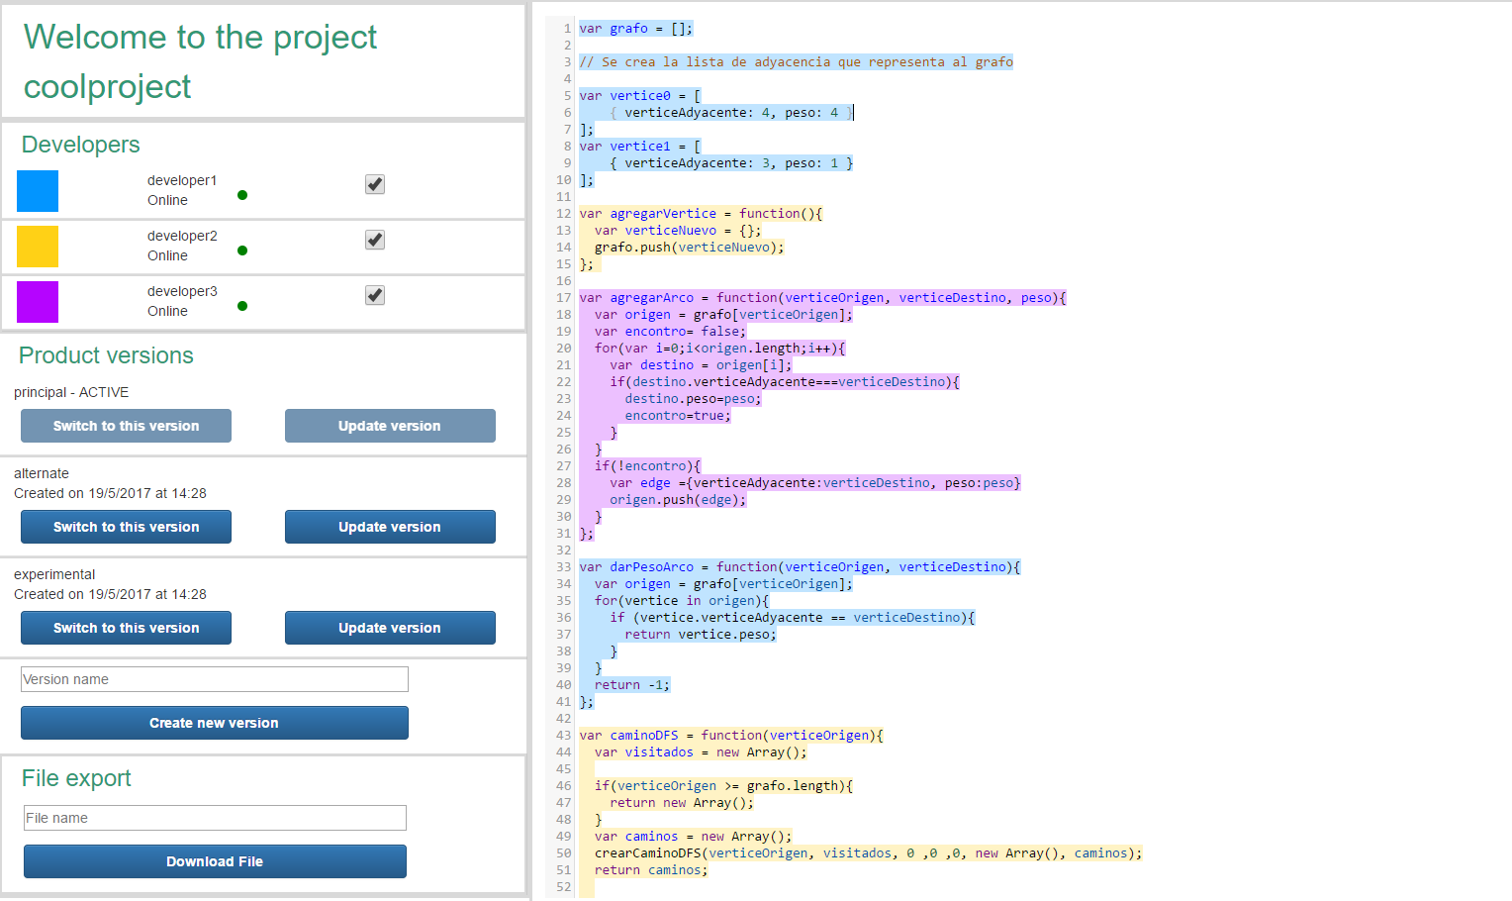
\includegraphics[width=0.7\textwidth]{img/fig1-collabIDEGeneral}
  \caption{CollabIDE tool}
  \label{fig:collabide}
\end{figure}

%%%%
\subsection{Experiment Setup}

\authorcomment[missing]{NC}{Tools, exercise}
	

%%%%
\subsection{Results}


%%%%
\subsection{Threads to Validity}



\endinput